\newpage
\genHeader

\section{Validate your installation with JUnit}

Did you notice the headings changed again? If you did, awesome! If not, we must emphasize viewing this handbook in a 'double paged' format to make changes clear. Remember, Red is Visual Syntax, Blue is Textual.

% Add 'Click arrow to change top level elements to working sets' here

\begin{itemize}

\item[$\blacktriangleright$] You should have a folder named ``DemoTestsuite .'' Right click on it to bring up the context menu and go to ``Run As / JUnit Test.'' If anything goes wrong, try refereshing your whole workspace by choosing each project and pressing  \texttt{F5}, or right-clicking and selecting ``Refresh.''

\vspace{0.5cm}

\begin{figure}[htbp]
	\centering
  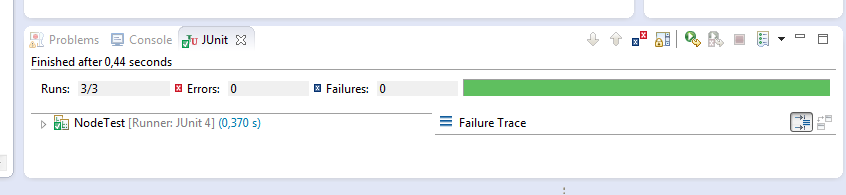
\includegraphics[width=1\textwidth]{eclipse_passedJUnitTest}
	\caption{All's well that ends well\ldots}
	\label{fig_passedTest}
\end{figure}

\vspace{0.5cm}

Congratulations!  If you see a green bar  (Fig.~\ref{fig_passedTest}), then everything has been set up correctly and you are now ready to start Metamodelling!

\end{itemize}

% Whitespace due to next section begins alternating between syntaxes again
\newpage
\mbox{}